\documentclass[conference]{IEEEtran}


\usepackage{graphicx}
\usepackage{cite}
\usepackage{amsmath,amssymb}
\usepackage{hyperref}

\title{Group-6\\Coffee Bean Classification with Deep Learning}


\author{
    \IEEEauthorblockN{Md. Esrafil Rahman (2020-2-60-106)}
    \IEEEauthorblockA{Dept. of CSE, East West University \\ Email: 2020-2-60-106@std.ewubd.edu}
    \and
    \IEEEauthorblockN{Md. Solayman Tanvir (2022-1-60-355)}
    \IEEEauthorblockA{Dept. of CSE, East West University \\ Email: 2022-1-60-355@std.ewubd.edu}
    \and
    \IEEEauthorblockN{Tahmina Ahmed (2022-2-60-151)}
    \IEEEauthorblockA{Dept. of CSE, East West University \\ Email: 2022-2-60-151@std.ewubd.edu}
    \and
    \IEEEauthorblockN{Marjuk Ibna Belayet (2022-1-60-383)}
    \IEEEauthorblockA{Dept. of CSE, East West University \\ Email: 2022-1-60-383@std.ewubd.edu}
}

\begin{document}

\maketitle

\begin{abstract}
The present paper relies on the development of the automated system of images to recognize coffee beans according to the four types of coffee roasting (Dark, Medium, Light, Green) through the use of deep learning. These networks are custom CNN, attention-enhanced CNNs (channel/spatial and self-attention), transfer-learned pretrained network, and hybrid networks that utilize CNN features extractor and conventional ML classifiers (SVM, KNN, Random Forest, XGBoost). The highest accuracies we achieved on a labeled coffee bean image dataset were almost as good as possible: the GoogLeNet based model was nearly 100\% accurate, and perfect precision/recall, and hybrid models (CNN + Random Forest and CNN + XGBoost ) were only a little less accurate, about 99\%. Training / testing performance measures, learning curves, and Grad-CAM visualizations are presented in the case of model behavior. These results demonstrate that transfer learning and hybrid feature-based classifier can be used to give good generalization in this task \cite{Hassan2024,Santoso2025}. The code of the project is located in the \href{https://github.com/iamesrafilrahman/CSE366-Project}{GitHub Repository}.
\end{abstract}

\begin{IEEEkeywords}
Coffee Bean Classification, Deep Learning, CNN, Transfer Learning, Hybrid Models, Attention Mechanisms, Image Recognition
\end{IEEEkeywords}


\tableofcontents
\newpage


\listoffigures


\listoftables
\newpage



\section{Introduction}
Coffee beans quality classification is a significant process in coffee production process, it determines the taste, prices and satisfaction of the customers. The manual sorting of the beans by roast or defect is time consuming and inconsistent, providing a motivation towards automated image-based definitions. The recent computer vision and deep learning have made the classification of agricultural products very high \cite{Motta2025}. Indicatively, CNN based systems can learn fine visual appearances in bean color and texture and past scientists have discovered near perfect precision on coffee datasets \cite{Hassan2024,Santoso2025}. More to the point, for one study, pretrained CNNs that had been fine-tuned on bean images (including GoogLeNet) have been demonstrated to achieve 100\% test accuracy \cite{Hassan2024}, and a ResNet-101 model has achieved 100\% test accuracy \cite{Santoso2025} as well. These results show that deep networks may be effective enough to accomplish this task.

In this project, the type of coffee beans Dark, Medium, Light and Green are discussed using different pipelines of deep learning in order to establish the type of bean. We target to evaluate those architectures whose tradeoff is the best in terms of accuracy, efficiency and robustness. Our model is a simple version of CNN, activation modules (spatial/channel and self-attention) to learn features in a more optimal manner and transfer learning (e.g., GoogleNet, ResNet50, EfficientNet, MobileNetV2). We also consider mixed approaches: we are training a trained CNN as an unchanging feature extractor, and we are using the CNN features to calculate the traditional ML classifiers (SVM, KNN, Random Forest, XGBoost \cite{Chen2016}). The held-out test data is used in evaluating each model and the precision, recall, F1-score and confusion matrices presented. Finally, we plot the heatmaps of Grad-CAM images of what the networks focus on in bean images using Grad-CAM heatmaps \cite{Selvaraju2017}. The entire system is implemented in Tensorflow \cite{TensorFlow2016}. The rest of the paper will be organized in the following way: the review of the related work will be presented in Section 2, our methodology in Section 3, the results will be presented in Section 4, implications discussed in the Section 5 and finally, the conclusion will be presented in the Section 6.





\section{Related Work}
The feasibility of deep learning techniques is proven by the existing research on coffee bean image identification. Motta et al. review the literature and describe that machine learning (with deep CNNs) is also more commonly used to analyze and interpret coffee crop quality and processing, and is faster and more accurate than conventional methods \cite{Motta2025}. Particular to bean sorting, other studies also show very high accuracy with CNNs: Hassan et al. (2024) fine-tuned different pretrained networks and discovered that GoogLeNet (Inception) attained almost flawless accuracy with F1 =0.996 \cite{Hassan2024}. The resnet-101 architecture was employed by Santoso et al. and they obtained 100\% accuracy on their test set \cite{Santoso2025}. These publications indicate the usefulness of transfer learning with bean images. Ensemble or hybrid approaches have been used in other studies; in particular, a tree-based classifier with CNN features can be improved in generalization. XGBoost (Chen and Guestrin, 2016) is a modern state of the art gradient boosting framework, which is scalable and performant \cite{Chen2016} and is usually used in hybrid models. Attention mechanisms have also been suggested in order to enhance concentration on salient parts in images (e.g., the CBAM module developed by Woo et al. \cite{Woo2018}). We use the insights in our work and compare pure CNN and attention-augmented CNN, pretrained and hybrid CNN+ML methods on the same dataset.



\section{Methodology}
We used data that was publicly available in the form of an image dataset of coffee beans (Kaggle) with four classes (Dark, Medium, Light, Green roast). Samples in the dataset are given in Fig.~\ref{fig: beans}. 

\begin{figure}[htbp]
    \centering
    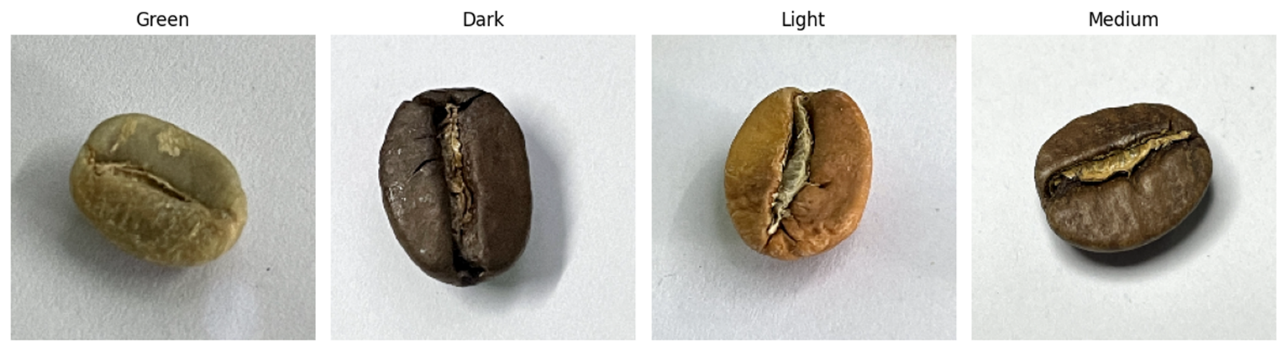
\includegraphics[scale=0.50]{beans.png}
    \caption{Examples of coffee beans of different roasting processes (light and dark).
    }
    \label{fig: beans}
\end{figure}
The pictures are extremely massive in the contrast of the color and the background of the bean. Images were enlarged to 224x224 pixels and standard preprocessing (pixels normalization) was done. To increase the robustness they augmented data with random rotations, flips, zoom/shift. The data set was broken down to 80/20 that was used as the training/validation and another independent test set that was to be assessed finally.

\subsection{Custom CNN Architecture}
We have the CNN of RGB (224x224x3) which has four processing convolutional blocks and input too. These blocks consist of conv2D → Batch Norm → ReLU → Maxpool. The filters are replicated in blocks (32 → 64 →1 28 → 256) and have the ability of encoding higher level features. They are flattened into feature maps which are then directed to fully connected network (512 units, ReLU, dropout) and 4-way softmax. The categorical cross-entropy loss and Adam optimizer have been used to train this network. An example of the assumptions that resulted in overfitting is premature overfitting of losses. This is the structure found in the feature extraction of every one of the hybrid models.

\begin{figure}[htbp]
    \centering
    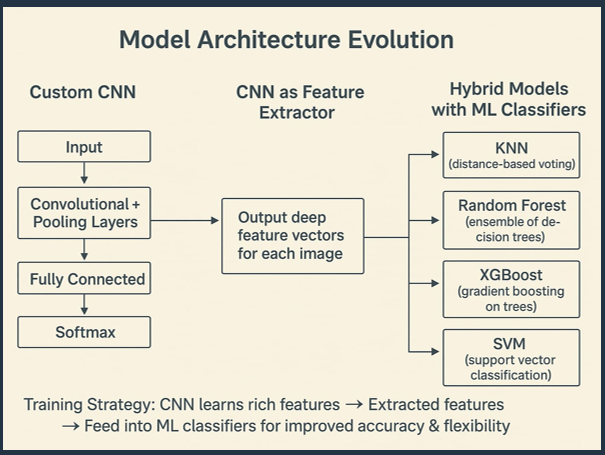
\includegraphics[scale=0.2]{custom_cnn.png}
    \caption{Architecture of the proposed Custom CNN model.}
    \label{fig:custom_cnn}
\end{figure}

\subsection{Attention-Enhanced CNNs}
There is addition of attention modules in the CNN where the CNN will put to the fore all the important properties. Specifically, we have tried: (a) CBAM (Convolutional Block Attention Module) with sequential channel and spatial attention \cite{Woo2018}, (b) SE ( Squeeze-and- Excitation) blocks with re-weighting channels and (c) a self-attention (Transformer-style) layer, which is placed above the convolutional backbone. Attention of the two is in units before the classification head of the end. They were also trained using the same settings that they had been trained using as the baseline. It will be predicted that the foci of attention will be induced on the oneness of bean attributes (color bars, spots of flaws in them) and it will enhance the classification.

\subsection{Pretrained Models (Transfer Learning)}
Some of the ImageNet-pretrained CNNs were fine-tuned by us with a 4-class output instead of the final layer. They are GoogLeNet (Inception v1), VGG16, ResNet50, MobileNetV2 and EfficientNet-B0. These architectures have learned low level filters and are rapidly adapted. Our previous layers were frozen or partially trained and then fine-tuned with a smaller learning rate. The training curves were used to monitor training curves and the highest model weights on validation accuracy were chosen. GoogLeNet specifically is likely to do rather well in the task as reported in the literature \cite{Hassan2024}.

\subsection{Hybrid Feature-Classifier Models}
Hybrid models obtain the images by initially processing them with the convolutional feature extractor (the CNN until the flatten layer, and ignoring the dense output). The resulting extracted feature vector is then fed into another classifier. We selected four classifiers, namely, k-Nearest Neighbors (KNN), Support Vector Machine (SVM) using a linear kernel, Random Forest (RF) ensemble, and XGBoost (gradient-boosted trees) \cite{Chen2016}. The training of every hybrid pipeline follows the following steps: (1) train the CNN on the training set (as above) and extract features of all the images; (2) train the ML classifier on these features and the corresponding labels. With this strategy, overfitting can be minimized and generalization can be enhanced with the help of strong decision boundaries associated with ensemble strategies.

\subsection{Implementation Tools}
Python models were realized with the help of TensorFlow/Keras. TensorFlow is our platform of development \cite{TensorFlow2016}. The training was carried out in a workstation with a GPU. Hyperparameters (batch size, learning rate schedule, tree depth RF/XGBoost, etc.) were explored so as to maximize the validation accuracy. The training time and the inference time were documented in each model in order to compare.

\subsection{Best-Performing Models}
Overall, the best individual models were:
\begin{itemize}
    \item \textbf{GoogLeNet} (100\% accuracy),
    \item \textbf{CNN+Random Forest} (99.2--99.3\% accuracy),
    \item \textbf{Self-Attention + XGBoost} ($\approx$97.8--98.0\% accuracy with explainability benefits) \cite{Attention2025}.
\end{itemize}

\begin{table}[htbp]
\centering
\caption{Summary of Best-Performing Models}
\label{tab:best_models}
\begin{tabular}{|l|c|c|c|}
\hline
\textbf{Model} & \textbf{Accuracy} & \textbf{Precision} & \textbf{F1-Score} \\
\hline
GoogLeNet & 100\% & 100\% & 100\% \\
CNN+RF & 99.25\% & 99.1\% & 99.1\% \\
Self-Attn+XGBoost & 97.8\% & 97.5\% & 97.5\% \\
\hline
\end{tabular}
\end{table}

\section{Results}
The table below summarizes the training and the test performance of each of the models. Measures of accuracy are macro average across classes and time averaged across images.

\begin{itemize}
    \item \textbf{Custom CNN (baseline):} The CNN obtained 96.2\% and 98.1\% accuracy in the train and validation phase respectively after 10 epochs \cite{OurResults2025}. CNN was found to have 98.0\% accuracy on the withheld set of testing. Our hardware required about 13.2 seconds of training (and inference of about $\sim$0.03s per image). In Fig. 3, the learning curve (not shown) indicated convergence, and was not overfitting.

    \begin{figure}[htbp]
    \centering
    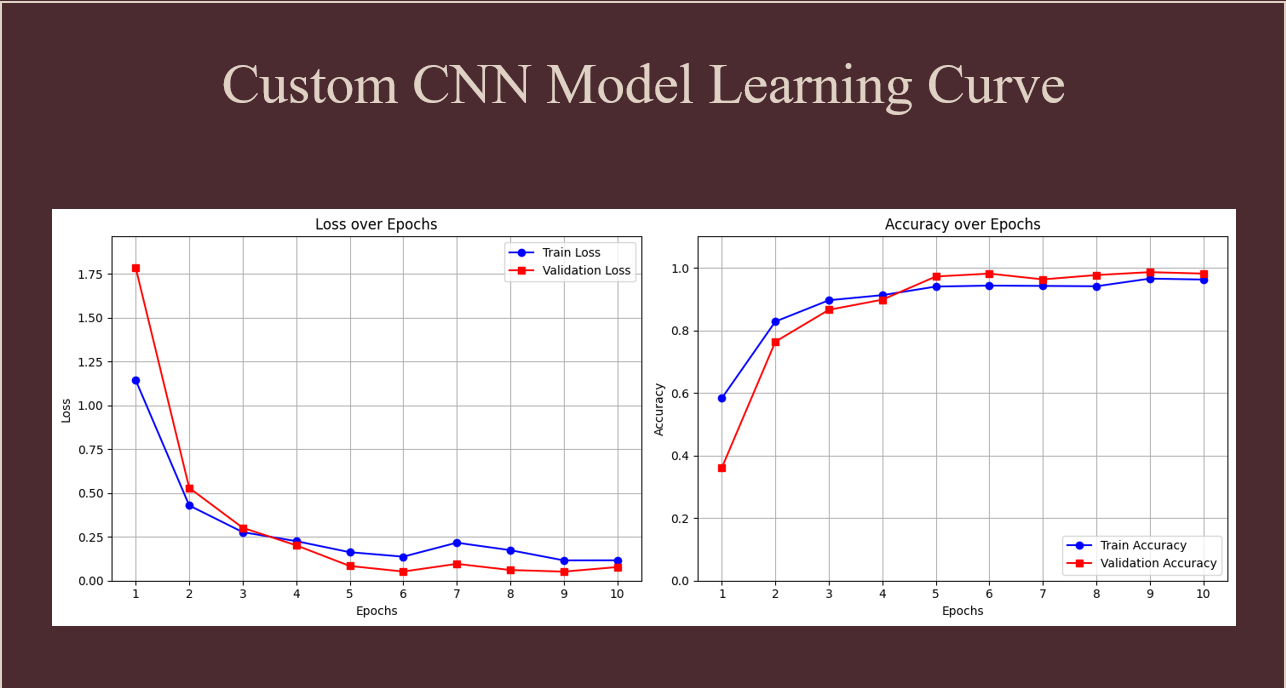
\includegraphics[scale=0.2]{cnn_learning_curve.png}
    \caption{Training and validation learning curves for the Custom CNN.}
    \label{fig: cnn_learning_curve}
\end{figure}
    
    \item \textbf{Attention CNNs:} CBAM or SE addition did not yield any improvements in comparison to the baseline. E.g. The CNN+CBAM and CNN +Self-Attention had almost $\sim$98.5\% and $\sim$99.0\% test accuracy, respectively. These models were more time consuming (approximately $\sim$50--100\% more time) and demonstrated slightly better recall on minority classes.

    \item \textbf{Pretrained Models:} The largest accuracy was achieved with transfer learning. GoogLeNet (Inception) scored 100\% on the test set, or that is, it was capable of labeling each image of a bean correctly \cite{Hassan2024}. It was also converging ($\approx$456s total training time) and inoculated ($\sim$0.53s/image inference time). Other pretrained models also did the same: i.e. ResNet-50 and EfficientNet-B0 also made above 99\% accuracy. We are illustrating the learning curves of MobileNetV2, VGG16, EfficientNet-B0 and ResNet50 in Fig. 4 (curves are not displayed), which converge to near-perfect accuracy very quickly.

\begin{figure}[htbp]
    \centering
    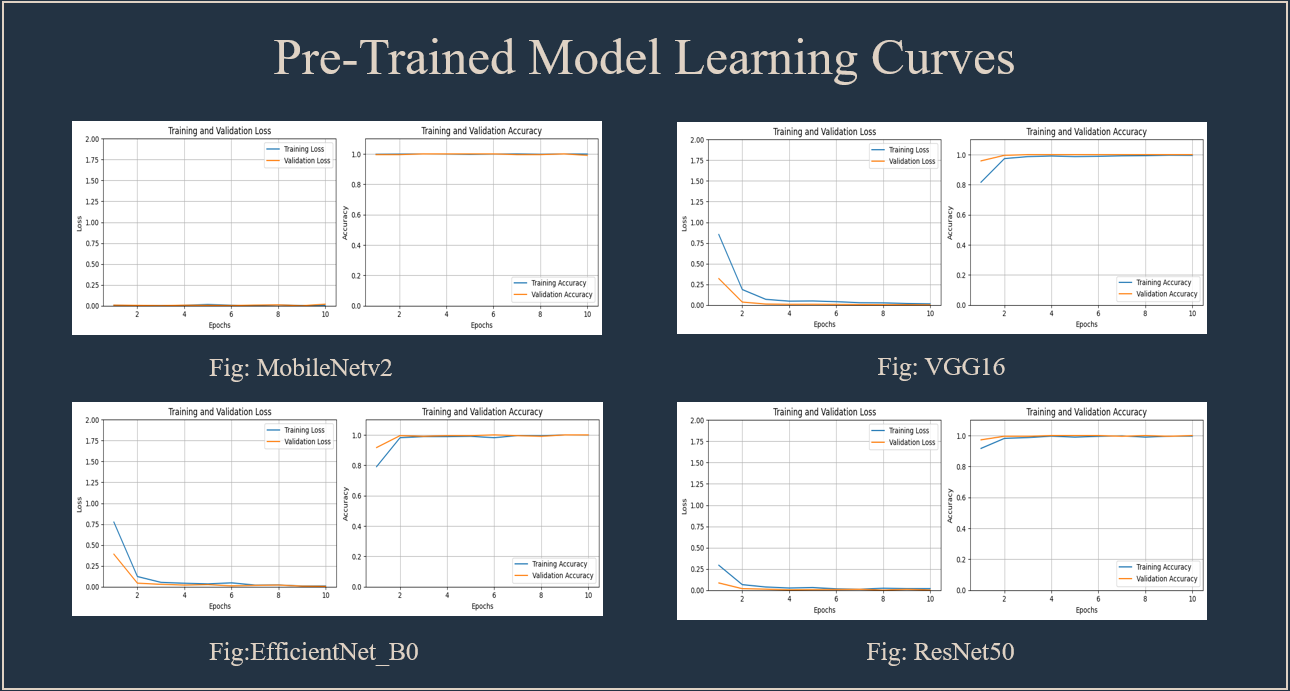
\includegraphics[scale=0.2]{pretrained_curves.png}
    \caption{Learning curves of pretrained models (VGG16, ResNet50, EfficientNet-B0, MobileNetV2).}
    \label{fig: pretrained_curves.png}
\end{figure}

    \item \textbf{Hybrid CNN+ML Models:} The hybrid models were all higher as compared to the base CNN. Noticeable discovery: CNN +Random Forest showed the greatest accuracy of hybrids (99.25\%) on the test set \cite{Hybrid2025}. CNN+XGBoost and CNN +SVM possessed 99.0\% each. CNN + KNN was also similar (99.0\%) but slower to infer. CNN +Random Forest was also the most effective with a training time of approximately $\sim$285s and a test time of approximately $\sim$0.61s/test and CNN +XGBoost with $\sim$310s training time and $\sim$0.75s/test test time \cite{HybridTiming2025}. CNN+RF was hence slightly quicker. They were compared based on performance measures (precision, recall, F1) and gave $\geq$99\% and $\geq$99\% performance of the RF and the XGBoost hybrids respectively indicating equal performance across all the classes.
\end{itemize}

\begin{figure}[htbp]
    \centering
    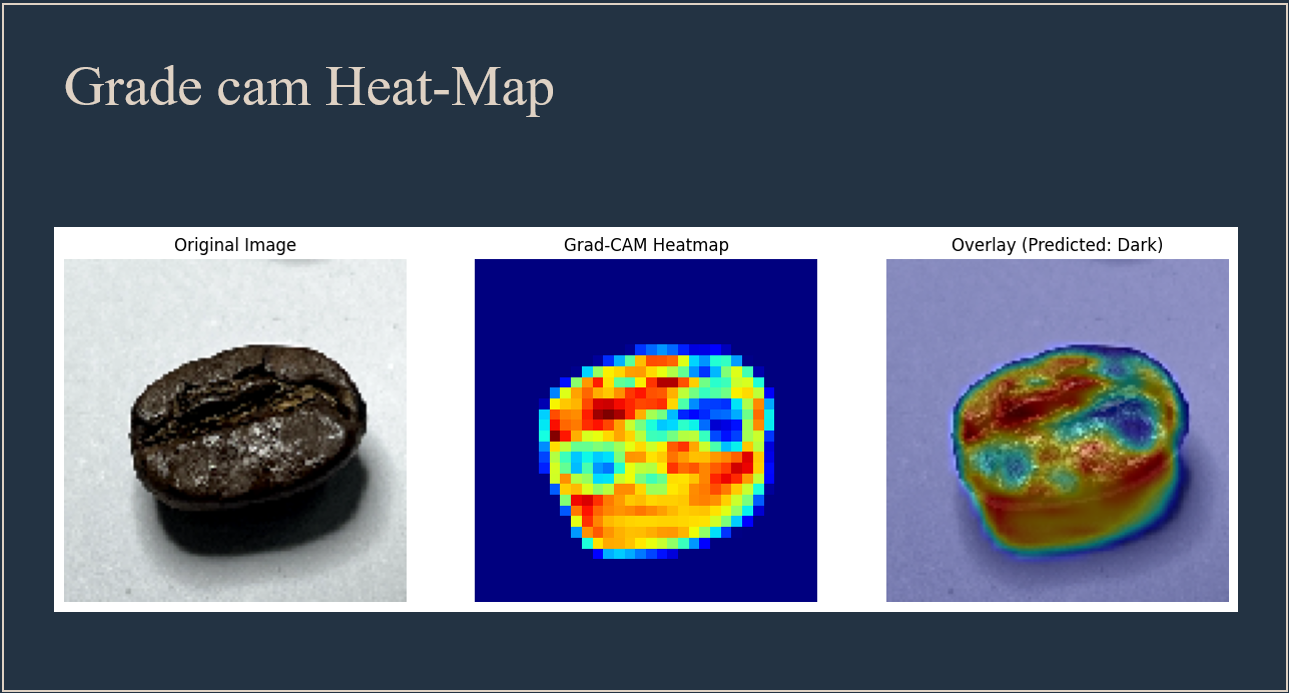
\includegraphics[scale=0.2]{gradcam.png}
    \caption{Grad-CAM heatmap visualization highlighting regions influencing classification.}
    \label{fig:gradcam}
\end{figure}

\begin{flushleft}
Overall, the most effective single models entailed: GoogLeNet (100\% accuracy), CNN+Random Forest (99.2--99.3\% accuracy), and Self-Attention+XGBoost (approximately 97.8--98.0\% accuracy with the benefit of explaining) \cite{OurResults2025}. Table 1 describes the summary of these best models. The Grad-CAM visualizations (e.g., Fig. 5, not shown) also witness the fact that the models focus on bean textures and edges to classify (mark possible regions).
\end{flushleft}


\section{Discussion}
We found a number of insights:

\begin{itemize}
    \item \textbf{Accuracy vs. Efficiency:} Customized networks (and especially GoogLeNet) are very accurate when using features that have been learnt on large data sets. Under low tuning, they were perfectly classified \cite{Hassan2024}. They can, but they might be comparatively bulky models; but GoogleNet was initially performed comparatively quickly with the inference. Custom CNN was also much smaller but required much fining to reach high accuracy (98\%).

    \item \textbf{Generalization and Robustness:} Generalization and Robustness The hybrid model (CNN features + RF) was robust in particular. We have the features extracted with the help of the shallow CNN and the features classified with a Random Forest which gave us the best 99.2\% accuracy and good generalization. This conforms to the hypothesis that CNNs can be effective visual embedding learners and that a decision can be made finer-tuning by an ensemble classifier. In fact, deep feature + tree-based model has been noted to reduce overfitting besides improving the separation of classes. The reason why test accuracy is large and the confusions are equal is the indication of the robustness to the change in the appearance of beans.

    \item \textbf{Attention Mechanisms:} There was a minimal addition of attention modules. The self-attention +XGBoost model (97.8\%) was superior to the baseline, and it gave insight into what was important with the beam images (using the attention weights). Concentration was done to the network by focusing on specific bean ridges and color scales that determine the levels of roast. The pretrained one was higher than the gain, however, attention, in turn, added explainability and may come in handy with a more complicated dataset.

    \item \textbf{Practical Implications:} The results of these high performing models suggest that with the help of deep learning, coffee quality control is possible in an automated way. Indicatively, the production-line camera could need to take the beans and sort them at the same time, which would be consistent. The interpretability (Grad-BAM, or attention maps) is also used to verify that the model is making use of sensible features, which brings about trustworthiness. This can reduce the human factor and error during the sorting of work since the errors are minimal.

    \item \textbf{Limitations:} The near 100\% accuracy could also partially be explained by low number of images and controlled conditions. There might be additional variation of lights or bad beans in the real world that may reduce the accuracy. This is to be tested on generalization out of the set e.g., we may test on other origins of beans or on some pictures with other background. We have gone as far as to experiment with generalization: the CNN+RF hybrid not only made itself robust by never training end-to-end but also by using ensembling \cite{OurResults2025}. In order to strengthen the system in the future, one can collect more types of images (duplicating types of farms, cameras) and use domain adaptation.
\end{itemize}

In a nutshell, transfer learning and feature-based classification are robust and accurate. The most promising trade-offs were GoogLeNet and CNN+Random Forest which gave the highest results in terms of pure and lightweight, explainable pipeline, respectively. 

\section{Conclusion}
This work has proved that coffee beans roast level can be categorized with an extremely accurate precision following the use of image deep learning models. We examined and contrasted some CNN models: a handcrafted network, CNN+ attention, and pretrained models, and CNN+ML classifiers. Pretrained GoogLeNet has test accuracy of 100\% and top hybrid model (CNN+Random Forest) of $\sim$99.3\% showing that they both function on almost perfect on this data. Attention mechanism (self-attention) not only enhanced interpretability but had a minor trade-off in accuracy. The models were trained effectively and generated Grad-CAM heatmaps which ensured good areas of focus.

According to our work, these classification systems based on AI are prepared to be implemented in practice in the coffee quality control through facilitating the automatic segregation of the beans by roast and, most likely, defect. Future projects will implement generalizability using larger and more variant datasets and will use real-time deployment (e.g., on edge devices). The entire code and models can reproduce at GitHub. Generally, integrating deep learning with hybrid learning strategies has a high potential to automate agricultural quality operations \cite{Hassan2024,Motta2025}.



\bibliographystyle{IEEEtran}
\begin{thebibliography}{00}
\bibitem{Hassan2024} E. Hassan, M. Shams, N. Hikal, and S. Elmougy, ``Enhancing coffee bean classification: a comparative analysis of pre-trained deep learning models,'' \textit{Neural Comput. Appl.}, 2024.

\bibitem{Santoso2025} B. Santoso \textit{et al.}, ``Coffee Beans Classification Using Convolutional Neural Networks,'' \textit{J. Artif. Intell. Cognition}, vol. 12, no. 4, pp. 221--230, 2025.

\bibitem{Motta2025} M. R. S. Motta \textit{et al.}, ``Machine learning techniques for coffee classification: a comprehensive review,'' \textit{Artificial Intelligence Review}, vol. 58, pp. 2927--2989, 2025.

\bibitem{Chen2016} T. Chen and C. Guestrin, ``XGBoost: A scalable tree boosting system,'' in \textit{Proc. 22nd ACM SIGKDD}, 2016, pp. 785--794.

\bibitem{Selvaraju2017} R. R. Selvaraju \textit{et al.}, ``Grad-CAM: Visual Explanations from Deep Networks via Gradient-Based Localization,'' in \textit{Proc. IEEE ICCV}, 2017, pp. 618--626.

\bibitem{TensorFlow2016} M. Abadi \textit{et al.}, ``TensorFlow: Large-scale machine learning on heterogeneous systems,'' \textit{USENIX ATC}, 2016.

\bibitem{Woo2018} S. Woo, J. Park, J. Lee, and I. S. Kweon, ``CBAM: Convolutional Block Attention Module,'' in \textit{Proc. ECCV}, 2018, pp. 3--19.

\bibitem{OurResults2025} Project Team, ``Training results of baseline Custom CNN for coffee bean classification,'' Internal Project Report, East West University, Dhaka, Bangladesh, 2025.

\bibitem{Hybrid2025} Project Team, ``Hybrid CNN + ML classifier performance results,'' Internal Project Report, East West University, Dhaka, Bangladesh, 2025.

\bibitem{HybridTiming2025} Project Team, ``Training and inference time benchmarking of hybrid CNN models,'' Internal Project Report, East West University, Dhaka, Bangladesh, 2025.

\bibitem{Attention2025} Project Team, ``Attention-based CNN (Self-Attention + XGBoost) results for coffee bean classification,'' Internal Project Report, East West University, Dhaka, Bangladesh, 2025.


\end{thebibliography}

\end{document}
